\section{Simulating Evolution}\label{sec:se}
In this section we cover how we represent microsatellites in this paper, the major different variations for simulation,
and the approach we take.

\subsection{Microsatellite Representation}\label{subsec:mr}
Let $\ell$ represent an integer associated with number of repeat units of a single microsatellite variation.
For example if we define our nucleotide sequence as $GATA$, the microsatellite variation below would represented
as $\ell=4$.
\begin{equation*}
    \ldots \mathit{GATAGATAGATAGATA} \ldots
\end{equation*}

In addition to $\ell$ being an integer, we also constrain $\ell$ to exist between some lower bound on repeat units
$\kappa$ and some upper bound $\Omega$.
Any $\ell_M$ that meets the criteria in~\autoref{eq:microsatelliteCriteria} is defined to be the repeat length associated
with some variant for the microsatellite $M$:
\begin{equation}\label{eq:microsatelliteCriteria}
    \left(\ell_M \in [\kappa, \Omega]\right) \land \left(\ell_M \in \mathbb{Z}\right)
\end{equation}

Let $\pi_t$ represent an $N$-sized tuple, or microsatellite \emph{population} of sequences
$\left(\ell_1, \ell_2, \ell_3, \ldots \ell_{N}\right)$ in a human population of size $\frac{N}{2}$ at generation $t$.
There exist two microsatellites variations per individual in a human population, but we relax the constraint that
each individual is associated with two sequences in $\pi_t$ for brevity.
The unit of interest here is the microsatellite variation itself, which moves through generations while collecting or
losing repeats until we are able to compare this to observed data.

%If at generation $t=1$, we have the population:
%\begin{equation}
%    \pi_1 = \left( \ell_1, \ell_2, \ell_3, \ell_4, \ell_5 \right)
%\end{equation}
%Our population for the next generation $t=2$ may comprise of the following:
%\begin{equation}
%    \pi_2 = \left( \ell_1, \ell_2, \ell_2, \ell_3, \ell_3\right)
%\end{equation}
%where individuals from the generation $t=1$ may not advance to the next generation $t=2$.
%In addition, there may exist duplicates from the previous generation.

\subsection{Forward Simulation}\label{subsec:fs}
There exists two main approaches toward which direction we should simulate toward: from the past to the present
(forward) or from the present to the past (backward).
In both cases, the goal is to create some evolutionary tree of $N$ microsatellites that trace back to some common
ancestor \emph{efficiently}.
In the section, we focus on forward simulation.

In order to simplify this problem, we assume the Wright-Fisher population model:
\begin{enumerate}
    \item Our population of sequences is of constant size $N$ for each generation.
    \item All individuals from some generation $t$ originate from the previous generation $t - 1$.
    \item There exists no selection bias, each sequence from the previous generation is equally likely to be
        chosen to exist in the next.
\end{enumerate}

\subsubsection{Evolving From $\pi_t$ To $\pi_{t+1}$}
Let $\pi_t$ represent a microsatellite population at generation $t$, of size $\left|\pi_t \right| = N$.
A forward simulation starts with population $\pi_0$, and evolves this population until all members of the current
population $\pi_{\bar{t}}$ shares a sole common ancestor.
Starting from $\pi_0$, under the Wright-Fisher model we generate $\pi_1$ by choosing $N$ individuals from $\pi_0$ with
replacement.
To generate $\pi_2$, we repeat the process to construct $\pi_1$ using $\pi_1$ instead of $\pi_0$.
This is repeated until we reach $\pi_{\bar{t}}$.

An example of the Wright-Fisher evolution process is given in~\autoref{fig:wrightFisherEvolution}.
Here, there exists two populations: a parent population $\pi_{t+1}$ and a child population $\pi_t$.


\begin{figure}
    \centering{\usetikzlibrary{arrows.meta}
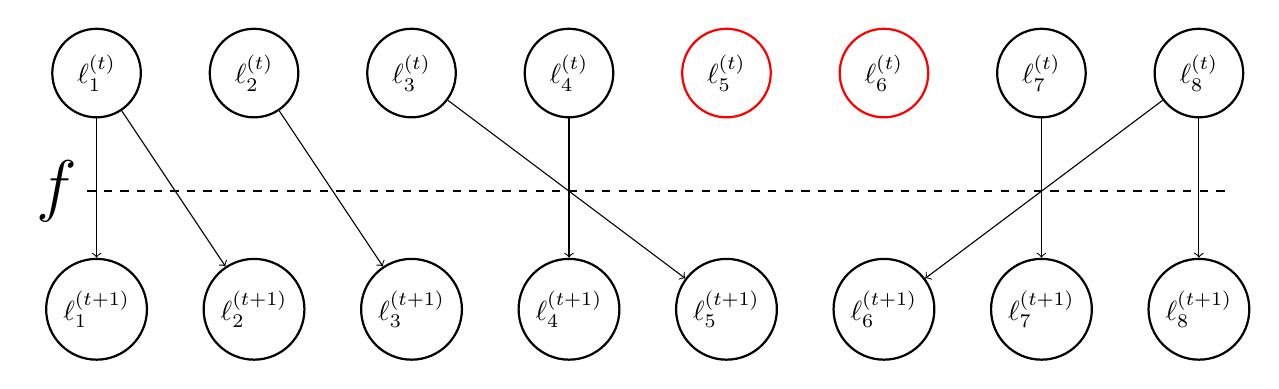
\begin{tikzpicture}
    \begin{scope}[auto, every node/.style={draw=black,circle,thick,minimum size=3.2em}]
        \node (A_1) at (0, 0) {$\ell^{(t + 1)}_1$};
        \node (A_2) at (2, 0) {$\ell^{(t + 1)}_2$};
        \node (A_3) at (4, 0) {$\ell^{(t + 1)}_3$};
        \node (A_4) at (6, 0) {$\ell^{(t + 1)}_4$};
        \node (A_5) at (8, 0) {$\ell^{(t + 1)}_5$};
        \node (A_6) at (10, 0) {$\ell^{(t + 1)}_6$};
        \node (A_7) at (12, 0) {$\ell^{(t + 1)}_7$};
        \node (A_8) at (14, 0) {$\ell^{(t + 1)}_8$};

        \node (B_1) at (0, 3) {$\ell^{(t)}_1$};
        \node (B_2) at (2, 3) {$\ell^{(t)}_2$};
        \node (B_3) at (4, 3) {$\ell^{(t)}_3$};
        \node (B_4) at (6, 3) {$\ell^{(t)}_4$};
        \node (B_7) at (12, 3) {$\ell^{(t)}_7$};
        \node (B_8) at (14, 3) {$\ell^{(t)}_8$};

        \node[draw=red] (B_5) at (8, 3) {$\ell^{(t)}_5$};
        \node[draw=red] (B_6) at (10, 3) {$\ell^{(t)}_6$};
    \end{scope}

    \begin{scope}
        \node (C_1) at (-0.5, 1.5) {\Huge$f$};
        \node (C_2) at (14.5, 1.5) {};
        \draw[thick, dashed] (C_1) -- (C_2);
    \end{scope}

    \begin{scope}[every edge/.style={draw=black}]
        \path[->] (B_1) edge (A_2);
        \path[->] (B_1) edge (A_1);
        \path[->] (B_2) edge (A_3);
        \path[->] (B_3) edge (A_5);
        \path[->] (B_4) edge (A_4);
        \path[->] (B_8) edge (A_6);
        \path[->] (B_8) edge (A_8);
        \path[->] (B_7) edge (A_7);
    \end{scope}
\end{tikzpicture}}
    \caption{An example of population $\pi_{t}$ evolving to $\pi_{t+1}$ under the Wright-Fisher model.}
    \label{fig:wrightFisherEvolution}
\end{figure}


\subsubsection{Average Time Until $N$ Individuals Coalesce: $\bar{t}$}
The next question that follows is, ``What is $\bar{t}$?''
The naive approach (but most correct) is to keep track of the evolutionary history for all populations.
This however requires (a) storage for the evolutionary tree formed and (b) an expensive search as we move forward for
each generation.
A compromise that avoids this search and storage increase is to fix $\bar{t}$ to some value, a time where most
populations have a common ancestor shared across the entire population.

In a Wright-Fisher population, the probability that any two individuals in $\pi_t$ share the same parent from
$\pi_{t-1}$ is:
\begin{equation}
    \begin{aligned}
        p(2, t-1) =& \frac{1}{N} \\
        q(2, t-1) =& 1 - \frac{1}{N}
    \end{aligned}
\end{equation}
where $p(2, t-1)$ represents the probability that two individuals share a parent from $\pi_{t-1}$ and
$q(2, t-1)$ represents the probability that two individuals do not share a parent from $\pi_{t-1}$.
The probability that two individuals do not share a parent in $\pi_{t-1}$, but do have a common ancestor
in $\pi_{t-2}$ is:
\begin{equation}
    p(2, t-2) = q(2, t-1) \cdot \frac{1}{N} = \frac{1}{N} \cdot \left(1 - \frac{1}{N}\right)
\end{equation}
If we ask the same question but for $\pi_{t-3}$, we get $p(2, t-3) = \frac{1}{N} \cdot  \left(1 - \frac{1}{N}\right)^2$.
Noting that $p$ is geometrically distributed, we can generalize $p$ for $y$ generations ago as such:
\begin{equation}
    p(2, t-y) = \frac{1}{N} \cdot \left(1 - \frac{1}{N}\right)^{y-1}
\end{equation}
with $p(2, t-y)$ having mean $E_2 = N$.
$E_2$ is interpreted as the expected number of generations until two individuals coalesce.

Now we look at the probability that \emph{three} individuals in $\pi_t$ share a parent from $\pi_{t-1}$.
Here, we asking how many pairs can be formed with $k=3$:
\begin{equation}
    p(3, t-1) = \frac{3}{N}
\end{equation}
Given $k=4$ individuals, the probability that any of the four share a parent in $\pi_{t-1}$ is
$p(4, t-1) = \frac{6}{N}$.
$p$ can be generalized for $k$ individuals:
\begin{equation}
    p(k, t-1) = \frac{\binom{k}{2}}{N}
\end{equation}
For $y$ generations, the general form of $p$ is given~\cite{hudsonGeneGenealogiesCoalescent1990}:
\begin{equation}
    p(k, t-y) = \frac{\binom{k}{2}}{N} \cdot \left(1 - \frac{\binom{k}{2}}{N}\right)^{y-1}
\end{equation}
with $p(k, t-y)$ having mean $E_k = \frac{N}{\binom{k}{2}}$.
$E_k$ is interpreted as the expected number of generations until $k$ individuals coalesce.

Going back to our original question, what is the average time until all $N$ individuals share a common ancestor?
Let us start with the average time until two individuals coalesce: $E_2 = N$ generations.
The average time until three individuals coalesce is the average time until any two individuals coalesce \emph{plus} the
average time until coalescence occurs in any three individuals.
For all $N$ individuals, this average time must be greater than:
\begin{equation}
    \bar{t} > \sum_{i=2}^{N} E_i \approx 2N
\end{equation}

\subsubsection{Algorithm for Forward Evolution}
The function  for forward evolution is presented in~\autoref{alg:forwardEvolution}.
There exists no applied mutation

\begin{algorithm}[ht]
    \SetAlgoLined
    \DontPrintSemicolon
    \Fn{SimulateForward \ {$(\ell^0, N, t_{epsilon})$}} {
        \KwIn{A common ancestor $\ell^0$, population size $N$, extra running time $t_\epsilon$}
        \KwOut{The resultant generation $\pi_{2N}$}
        $\pi_{t-1} \gets $ an $N$ sized vector, whose values are all set to $\ell^0$ \;
        $\pi_t \gets $ an empty $N$ sized vector \;
        \For{$i \gets 2$ \KwTo $t_\epsilon + 2N$} {
            \For{$j \gets 1$ \KwTo $N$} {
                $\pi_t[j] \gets $ a randomly selected $\ell$ from $\pi_{t-1}$ \;
            }
            $\pi_{t-1} \gets \pi_t$ \;
            $\pi_t \gets$ an empty $N$ sized vector \;
        }
        \Return $\pi_{t-1}$ \;
    }
    \textbf{end} \;
    \caption{Generate a population of individuals who \emph{likely} share some common
    ancestors.}\label{alg:forwardEvolution}
\end{algorithm}

\subsection{Backward Simulation}\label{subsec:bs}
Forward simulation has the advantage of being incredibly straightforward to implement and apply complex generation to
generation models to.
The biggest disadvantage with this type of simulation though, is that (1) $2N^2$ individuals must be generated and
(2) several returned populations from

\begin{figure}
    \centering
    \subfloat{{ \usetikzlibrary{decorations.pathreplacing}
\begin{tikzpicture}
    \begin{scope}[auto, every node/.style={draw=black,circle,thick,minimum size=1em}]
        \foreach \x in {1,...,5}
            \foreach \y in {0,...,8}{
                \node (\x\y) at (\x,\y) {};
            }
    \end{scope}

    \begin{scope}[auto, every node/.style={draw=black,circle,thick,minimum size=1em,fill=blue}]
        \node (A_1) at (3,0) {};
        \node (A_2) at (5,0) {};

        \node (B_1) at (1,1) {};
        \node (B_2) at (4, 1) {};

        \node (C_1) at (2, 2) {};
        \node (C_2) at (5, 2) {};

        \node (D_1) at (2, 3) {};
        \node (D_2) at (3, 3) {};

        \node (E_1) at (3, 4) {};
        \node (F_1) at (1, 5) {};
        \node (G_1) at (4, 6) {};
        \node (H_1) at (2, 7) {};
        \node (I_1) at (3, 8) {};
    \end{scope}

    \begin{scope}[every edge/.style={draw=black,thick}]
        \path (A_1) edge (B_1);
        \path (A_2) edge (B_2);
        \path (B_1) edge (C_1);
        \path (B_2) edge (C_2);
        \path (C_1) edge (D_1);
        \path (C_2) edge (D_2);
        \path (D_1) edge (E_1);
        \path (D_2) edge (E_1);

        \path (E_1) edge (F_1);
        \path (F_1) edge (G_1);
        \path (G_1) edge (H_1);
        \path (H_1) edge (I_1);
    \end{scope}

    \node (T_A) at (0.5, -0.25) {};
    \node (T_B) at (0.5, 4.25) {};
    \draw[decoration={calligraphic brace,amplitude=10pt},decorate,line width=1.2pt]
    (T_A) -- node[anchor=east, xshift=-8pt] {$\bar{t} = N$} (T_B);
\end{tikzpicture} }}
    \qquad \qquad \qquad
    \subfloat{{ \usetikzlibrary{decorations.pathreplacing}
\begin{tikzpicture}
    \begin{scope}[auto, every node/.style={draw=black,circle,thick,minimum size=1em,fill=blue}]
        \node (A_1) at (1,0) {};
        \node (A_2) at (5, 0) {};
        \node (A_3) at (3, 4) {};
    \end{scope}

    \begin{scope}[every edge/.style={draw=black,thick}]
        \path (A_1) edge (A_3);
        \path (A_2) edge (A_3);
        \node (A_4) at (3, 8.5) {};
        \path (A_3) edge (A_4);
    \end{scope}

    \node (T_A) at (0.5, -0.25) {};
    \node (T_B) at (0.5, 4.25) {};
    \draw[decoration={calligraphic brace,amplitude=10pt},decorate,line width=1.2pt]
    (T_A) -- node[anchor=east, xshift=-8pt] {$\bar{t} = N$} (T_B);
\end{tikzpicture} }}
    \caption{A coalescent buried in some forward simulation.}
    \label{fig:coalescentBuried}
\end{figure}

\begin{figure}
    \centering
    \usetikzlibrary{decorations.pathreplacing}
\begin{tikzpicture}[scale=0.65]
    \begin{scope}[auto, every node/.style={draw=black,circle,thick,minimum size=1em,fill=blue}]
        \node (A_1) at (1, 0) {};
        \node (A_2) at (2, 0) {};
        \node (A_3) at (3, 0) {};
        \node (A_4) at (4, 0) {};
        \node (A_5) at (5, 0) {};

        \node (B_1) at (1.5, 0.5*1.2) {};  % N = 5, 5 choose 2 = 10, 5 / 10 = 0.5
        \node (B_2) at (2.5, 0.5*1.2) {};
        \node (B_3) at (3.5, 0.5*1.2) {};
        \node (B_4) at (4.5, 0.5*1.2) {};

        \node (C_1) at (2, 1.33*1.2) {};  % N = 5, 4 choose 2 = 6, 5 / 6 = 0.83
        \node (C_2) at (3, 1.33*1.2) {};
        \node (C_3) at (4, 1.33*1.2) {};

        \node (D_1) at (2.5, 3*1.2) {};  % N = 5, 3 choose 2 = 3, 5 / 3 = 1.66
        \node (D_2) at (3.5, 3*1.2) {};

        \node (E_1) at (3, 8*1.2) {};  % N = 5, 2 choose 2 = 1, 5 = 5
    \end{scope}

    \begin{scope}[every edge/.style={draw=black,thick}]
        \path (A_1) edge (B_1);
        \path (A_2) edge (B_1);
        \path (A_3) edge (B_2);
        \path (A_4) edge (B_3);
        \path (A_5) edge (B_4);

        \path (B_1) edge (C_1);
        \path (B_2) edge (C_1);
        \path (B_3) edge (C_2);
        \path (B_4) edge (C_3);

        \path (C_1) edge (D_1);
        \path (C_2) edge (D_1);
        \path (C_3) edge (D_2);

        \path (D_1) edge (E_1);
        \path (D_2) edge (E_1);
    \end{scope}

    \node (T_A) at (0.5, -0.25) {};
    \node (T_B) at (0.5, 0.6+0.25) {};
    \draw[decoration={calligraphic brace,amplitude=2pt},decorate,line width=1.2pt]
    (T_A) -- node[anchor=east, xshift=-8pt] {$t_4$} (T_B);

    \node (T_B2) at (0.5, 0.6) {};
    \node (T_C) at (0.5, 1.6+0.25) {};
    \draw[decoration={calligraphic brace,amplitude=2pt},decorate,line width=1.2pt]
    (T_B2) -- node[anchor=east, xshift=-8pt] {$t_3$} (T_C);

    \node (T_C2) at (0.5, 1.6) {};
    \node (T_D) at (0.5, 3.6+0.25) {};
    \draw[decoration={calligraphic brace,amplitude=2pt},decorate,line width=1.2pt]
    (T_C2) -- node[anchor=east, xshift=-8pt] {$t_2$} (T_D);

    \node (T_D2) at (0.5, 3.6) {};
    \node (T_E) at (0.5, 9.6+0.25) {};
    \draw[decoration={calligraphic brace,amplitude=2pt},decorate,line width=1.2pt]
    (T_D2) -- node[anchor=east, xshift=-8pt] {$t_1$} (T_E);
\end{tikzpicture}
    \caption{A coalescent tree.}
    \label{fig:coalescentTree}
\end{figure}